% Options for packages loaded elsewhere
\PassOptionsToPackage{unicode}{hyperref}
\PassOptionsToPackage{hyphens}{url}
%
\documentclass[
]{article}
\usepackage{amsmath,amssymb}
\usepackage{lmodern}
\usepackage{iftex}
\ifPDFTeX
  \usepackage[T1]{fontenc}
  \usepackage[utf8]{inputenc}
  \usepackage{textcomp} % provide euro and other symbols
\else % if luatex or xetex
  \usepackage{unicode-math}
  \defaultfontfeatures{Scale=MatchLowercase}
  \defaultfontfeatures[\rmfamily]{Ligatures=TeX,Scale=1}
\fi
% Use upquote if available, for straight quotes in verbatim environments
\IfFileExists{upquote.sty}{\usepackage{upquote}}{}
\IfFileExists{microtype.sty}{% use microtype if available
  \usepackage[]{microtype}
  \UseMicrotypeSet[protrusion]{basicmath} % disable protrusion for tt fonts
}{}
\makeatletter
\@ifundefined{KOMAClassName}{% if non-KOMA class
  \IfFileExists{parskip.sty}{%
    \usepackage{parskip}
  }{% else
    \setlength{\parindent}{0pt}
    \setlength{\parskip}{6pt plus 2pt minus 1pt}}
}{% if KOMA class
  \KOMAoptions{parskip=half}}
\makeatother
\usepackage{xcolor}
\usepackage[margin=1in]{geometry}
\usepackage{longtable,booktabs,array}
\usepackage{calc} % for calculating minipage widths
% Correct order of tables after \paragraph or \subparagraph
\usepackage{etoolbox}
\makeatletter
\patchcmd\longtable{\par}{\if@noskipsec\mbox{}\fi\par}{}{}
\makeatother
% Allow footnotes in longtable head/foot
\IfFileExists{footnotehyper.sty}{\usepackage{footnotehyper}}{\usepackage{footnote}}
\makesavenoteenv{longtable}
\usepackage{graphicx}
\makeatletter
\def\maxwidth{\ifdim\Gin@nat@width>\linewidth\linewidth\else\Gin@nat@width\fi}
\def\maxheight{\ifdim\Gin@nat@height>\textheight\textheight\else\Gin@nat@height\fi}
\makeatother
% Scale images if necessary, so that they will not overflow the page
% margins by default, and it is still possible to overwrite the defaults
% using explicit options in \includegraphics[width, height, ...]{}
\setkeys{Gin}{width=\maxwidth,height=\maxheight,keepaspectratio}
% Set default figure placement to htbp
\makeatletter
\def\fps@figure{htbp}
\makeatother
\setlength{\emergencystretch}{3em} % prevent overfull lines
\providecommand{\tightlist}{%
  \setlength{\itemsep}{0pt}\setlength{\parskip}{0pt}}
\setcounter{secnumdepth}{5}
\newlength{\cslhangindent}
\setlength{\cslhangindent}{1.5em}
\newlength{\csllabelwidth}
\setlength{\csllabelwidth}{3em}
\newlength{\cslentryspacingunit} % times entry-spacing
\setlength{\cslentryspacingunit}{\parskip}
\newenvironment{CSLReferences}[2] % #1 hanging-ident, #2 entry spacing
 {% don't indent paragraphs
  \setlength{\parindent}{0pt}
  % turn on hanging indent if param 1 is 1
  \ifodd #1
  \let\oldpar\par
  \def\par{\hangindent=\cslhangindent\oldpar}
  \fi
  % set entry spacing
  \setlength{\parskip}{#2\cslentryspacingunit}
 }%
 {}
\usepackage{calc}
\newcommand{\CSLBlock}[1]{#1\hfill\break}
\newcommand{\CSLLeftMargin}[1]{\parbox[t]{\csllabelwidth}{#1}}
\newcommand{\CSLRightInline}[1]{\parbox[t]{\linewidth - \csllabelwidth}{#1}\break}
\newcommand{\CSLIndent}[1]{\hspace{\cslhangindent}#1}
\usepackage{amstext}
\usepackage{amsmath}
\usepackage{booktabs}
\usepackage{longtable}
\usepackage{array}
\usepackage{multirow}
\usepackage{wrapfig}
\usepackage{float}
\usepackage{colortbl}
\usepackage{pdflscape}
\usepackage{tabu}
\usepackage{threeparttable}
\usepackage{threeparttablex}
\usepackage[normalem]{ulem}
\usepackage{makecell}
\usepackage{xcolor}
\usepackage{algorithm,algorithmic}
\AtBeginEnvironment{CSLReferences}{\small}
\usepackage{tabularx}
\ifLuaTeX
  \usepackage{selnolig}  % disable illegal ligatures
\fi
\IfFileExists{bookmark.sty}{\usepackage{bookmark}}{\usepackage{hyperref}}
\IfFileExists{xurl.sty}{\usepackage{xurl}}{} % add URL line breaks if available
\urlstyle{same} % disable monospaced font for URLs
\hypersetup{
  pdftitle={Directed topic extraction with side information for sustainability analysis},
  pdfauthor={Maria Osipenko},
  hidelinks,
  pdfcreator={LaTeX via pandoc}}

\title{Directed topic extraction with side information for sustainability analysis}
\author{Maria Osipenko}
\date{2024-02-19}

\begin{document}
\maketitle

\hypertarget{abstract}{%
\section{Abstract}\label{abstract}}

Topic analysis represents each document of a text corpus in a low dimensional latent topic space. In some cases the desired topic representation is subject to specific requirements or guidelines constituting side information. For instance, sustainability aware investors might be interested in automatically assessing firm sustainability aspects from textual content of corporate reports with a focus on the established 17 UN sustainability goals. The main corpus here contains the corporate report texts, and the texts with the definitions of the 17 UN sustainability goals represent the side information. Under assumption that both text corpora share a common low dimensional subspace, we propose to represent them in a such via directed topic extraction by matrix co-factorization. Both, the main and the side text corpora are first represented as term-document matrices, which are then jointly decomposed into word-topic and topic-document matrices. Thereby, the word-topic matrix is common to both text corpora, whereas the topic-document matrices contain specific representations in the shared topic space. A nuisance parameter, which allows to move focus between error minimization of individual factorization terms, controls the extent, to which the side information is taken into account. With our approach, documents from the main and the side corpora can be related to each other in the resulting latent topic space. That is, the considered corporate reports are represented in the same latent topic space as the descriptions of the 17 UN sustainability goals, such that a structured automatic sustainability assessment of textual reports content is possible. We provide an algorithm for such directed topic extraction and propose techniques for visualizing and interpreting the results.

\hypertarget{introduction}{%
\section{Introduction}\label{introduction}}

The market for sustainable investments grows steadily. However, there are no uniform standards for comparing/quantifying sustainability levels of firms. Although several agencies provide in the mean time environmental, social, governance (ESG) rating, Berg, Kölbel, and Rigobon (2022) points out the disagreement of such ratings across the rating agencies. In this situation, it seems hard to overview the ESG development of potential investment firms and decide upon investors ESG value system.

In the same time, large companies communicate their ESG related strategy and actions in their sustainability reporting in form of:

\begin{itemize}
\item
  corporate responsibility reports
\item
  sustainability reports
\item
  environmental action reports
\end{itemize}

or similar sustainability related reports. The intention of such reporting is to increase the transparency and accountability of ESG related company actions for the stakeholders as Soh (2014).

Analysis of sustainability related textual sources have captured attention of numerous researches. To incorporate the specifics of sustainability texts, authors mainly rely on hand-crafted concepts and keywords. For instance, Liew, Adhitya, and Srinivasan (2014) use word and phrase frequencies to extract common trends and their importance from sustainability reporting based on sustainability content trees. Using their five content categories and the associated keywords, Landrum and Ohsowski (2017) perform content analysis of sustainability related corporate reports based on the proportion of the contained keywords.
Tsalis et al. (2020) propose to evaluate the level of alignment of sustainability related reports with an an established systematic - commonly accepted 17 UN sustainable development goals (SDGs, \url{https://sdgs.un.org/goals}). SDGs represent intergovernmental set of 17 goals which broadly address modern environmental and social challenges adopted in 2015 by the UN General Assembly. The goal is to structure the information from textual sustainability reports with the respect to the SDGs in a way, which enables a sound comparison of companies' contribution to solving those major challenges. Tsalis et al. (2020) use a scoring system based on disclosure topics from Global Reporting Initiative. They create a catalog of disclosure topics with respect to the SDGs using their expertise and the previous research, and use a scoring system to manually assign a score for each report with a view to each of the catalog items, which they aggregate at the end.

A common draw back of the works is the extended usage of human expertise in the analysis, which reduces the objectivity of the results on one hand and is time consuming on the the other.

The authors in Kang and Kim (2022) propose to assess textual information in sustainability related reports using SDGs as an anchor fully automatically. They choose sentence similarity method to assess the relatedness of the reports to the goals. The approach of Kang and Kim (2022) is computationally intensive, because each sentence in a report has to be compared to each sentence of a SDG text, and does not provide a transparent report representation with low complexity, such as a representation in a low dimensional topic space. The authors explain, that they reject the classical word frequency-based topic analysis, used in previous research, because it can not incorporate any ``predefined theme structure''. In this paper, we overcome the limitations proposeíng a topic analysis method using co-matrix factorization which integrates any predefined structure into the analysis. Our method leverages information from the textual sources on sustainability via automatic topic extraction while considering the value system established by the 17 SDGs and thus provides a low dimensional topic representation convenient for asssessing the level of association between the SDGs and sustainability related reports.

Topic analysis (Churchill and Singh (2022)) represents each document in a collection of documents in a low dimensional latent topic space. The most popular classical methods are Latent (probabilistic) semantic analysis (Deerwester et al. (1990), Hofmann (1999)), Latent Dirichlet allocation (LDA, Blei, Ng, and Jordan (2003)) as well as general purpose dimension reduction methods as non-negative matrix factorization (NMF, Lee and Seung (2000), Vangara et al. (2020)), and extensions of the methods above (e.g.~in Yang and Li (2015/07), Suleman and Korkontzelos (2021), and Figuera and García Bringas (2024)). Recently, also deep neural network based models have been proposed (Zhao et al. (2021)).

Topic extraction for structuring text data has been used extensively used in financial literature. For instance, Li et al. (2017) employ Latent Dirichlet Allocation (LDA) to structure financial stability reports. Yu Chen et al. (2017) compares Principal component analysis, NMF, LDA and deep learning models for text analytics in banking. Amini, Bienstock, and Narcum (2018) perform automatic topic extraction using the common methods for sustainability related reports specifically. W. Chen et al. (2023) uses LDA and neural network based models to analyse news impact on financial markets. For a comprehensive review of text mining and topic analysis in finance literature, we refer to Loughran and McDonald (2016) and Gupta et al. (2020). Despite the popularity of LDA, Yong Chen et al. (2019) and Egger and Yu (2022) argue, that NMF can outperform the latter by extracting interpretable topics, especially for short texts. Since we are going to cut the reports into small peaces of context, NMF is a promising technique for our needs. Moreover, Nugumanova et al. (2022) highlights the advantage of NMF-based methods for efficient extraction of domain specific terms, which is also relevant for our task with sustainability focus.

Recently, several LDA-based topic extraction methods that allow to explicitly embed known structure or side information have been proposed. For instance, Harandizadeh, Priniski, and Morstatter (2022) proposes to use word2vec embeddings combined with LDA and vocabulary priors to obtain interpretable word embeddings. Eshima, Imai, and Sasaki (2023) embed prespecified keywords in LDA for the same reason. In the same spirit, Watanabe and Zhou (2022) use seeded LDA with a carefuly chosen seeded vocabulary to assist in classifying documents in specific categories. With their approaches, the authors account for additional information in topic extraction. The draw back of the mentioned approaches in Watanabe and Zhou (2022) and Eshima, Imai, and Sasaki (2023) lies in the need of manual intervention for keyword or vocabulary specification. Harandizadeh, Priniski, and Morstatter (2022) uses word vectors from a pretrained general purpose word2vec model and thus, it is not clear, whether their model works for specific domains as sustainability reports.

On the other hand, there exist matrix factorization based approaches which integrate side information into dimension reduction. Rao et al. (2015) and later Zhang et al. (2020) propose to integrate side information using graphs. They derive a graph regularized version of matrix factorization and an associated alternating algorithm. However, their side information is not high dimensional and incorporates few individual characteristics which build basis for the graph links. Yet another way to consider high dimensional additional information are matrix co-factorization techniques.
Co-factorization techniques factorize two or three matrices with some common cofactors simultaneously. For instance, Fang and Si (2011) consider user communities information and Luo et al. (2019) incorporate tagging and time stamp of ratings in their personalized recommendations via matrix co-factorization. The approach is transparent and easily adjustable. By introducing a nuisance parameter which allows to move the focus between error minimization of individual factorization terms, additional flexibility is ensured.

In this paper, we propose a topic model based on non-negative matrix co-factorization (NMCF) to extract sustainability related topics from the related textual sources with the 17 UN goals as side information. The advantages of our approach include a fully automated topic extraction (without manual key word search), its interpretability, its adaptivity (via nuisance parameter \(\lambda\)), and a simple, scalable implementation.

The paper is structured as follows. In the next chapter, we explain the method used and derive the NMCF algorithm for topic extraction with side information. We also introduce the data in form of sustainability related reporting and the 17 UN goals, and describe our preprocessing steps. The results of the application of our algorithm to the data follow. Finally, we conclude and discuss future research directions.

\hypertarget{data-and-methods}{%
\section{Data and Methods}\label{data-and-methods}}

In this section, we introduce our data basis and describe the preprocessing steps. Subsequently, we present our method of non-negative matrix co-factorization (NMCF) and derive the NMCF algorithm for topic extraction with side information.

\hypertarget{data-and-preprocessing}{%
\subsection{Data and preprocessing}\label{data-and-preprocessing}}

Large listed companies disclosure their sustainability related actions in the associated corporate responsibility reports, sustainability reports or similar releases on a regular basis. These reports are aimed to increase transparency and disclosure sustainability awareness of the companies. A typical report contains many pages with rather a short message on a sustainability action and related pictures.

We use corporate responsibility/sustainability reports of top eight listed tech companies with tickers: AAPL, AMZ, DELL, GOOG, IBM, INTC, MSFT, and SSU. The associated time period includes the years 2013 (or later) to 2022 depending on the availability. The entities in the resulting main text corpus are the pages of the reports.

Our side information are the texts of the 17 UN SDGs which we obtain from the UN Website (\url{https://sdgs.un.org/goals}). The entities in the side information text corpus are the texts of the individual goals description.

All calculations are done in R (R Core Team (2023)). For the preprocessing on word level, we use R-Package Quanteda (Benoit et al. (2018)) to set up a corpus, to split in tokens, and compute the relative frequencies. We, first, structure our text corpora in the bag-of-words fashion (with two-grams as terms) and construct the term-context representations with the pooled vocabulary on this basis. In the next step, we combine the term in a common dictionary, such that our bag-of-words representation contains all relevant terms,

\hypertarget{non-negative-matrix-co-factorization-for-sustainability-analysis}{%
\subsection{Non-negative matrix co-factorization for sustainability analysis}\label{non-negative-matrix-co-factorization-for-sustainability-analysis}}

We assume that the corporate reports texts share a common topic structure with the sustainability goals definition but also contain some other topics concerning e.g.~financial statements. Moreover, we anticipate that the goals are written very focused using concrete sparse vocabulary, whereas the reports may refer to the same concepts using other wordings. That is, a common topic may contain words that are semantically relevant to sustainability goals vocabulary but not directly mentioned in the texts of the SDGs.
That is, we assume, that both text corpora share a common low dimensional subspace, in which they can be compared to each other by means of some distance measure.

To account for the mentioned issues, we define the following model for terms-document matrices arising from reports and sustainability goals texts.

\[M = U^\top V + E\]

and

\[C = U^\top Q + F\]

where

\begin{itemize}
\tightlist
\item
  \(M\) is the (weighted) term-context matrix for the corporate reports with dimensions \((p\times n)\), where \(p\) is the joint vocabulary (words and phrases with two co-occurring words) obtained from both reports and sustainability goals texts. \(n\) is the number of corporate reports contexts, where the later represents one page of a corporate report.
\item
  \(C\) is the (weighted) term-context matrix for the sustainability goals with dimensions \((p\times m)\), where \(p\) is again the joint vocabulary (words and phrases with two co-occurring words) obtained from both reports and sustainability goals texts. \(m\) is the number of sustainability goals contexts, where each context represents each of the \(17\) goals.
\item
  \(U\) is the term-topic representation matrix of dimensions \((p\times K)\), where \(K\) is the number of common topics and \(K\leq \min(rank(M),rank(C))\) is the number of topics.
\item
  \(V\) is the context-topic representation matrix for the reports of dimensions \((K\times n)\).
\item
  \(Q\) is the context-topic representation matrix for sustainability goals of dimensions \((K\times m)\).
\item
  \(E\) and \(F\) are matrices of error terms of dimensions \((p\times n)\) and \((p\times m)\) respectively.
  The overall dimensions for our data are \(p=18,086\) and \(n=6,891\).
\end{itemize}

The associated topic extraction problem is then:

\begin{equation}\min(||M - U^\top V||^2 + \lambda ||C-U^\top Q||^2)\label{eq:minc}
\end{equation}

where \(\lambda\) adapts the importance of the loss on the second factorization term (see Figure for a schematic representation of the approach).
The value of \(\lambda\) balances out the combined loss function. It is responsible for adjusting the impact of accuracy concerning reports versus SDGs. Since the second dimension of \(C\) is much lower than that of \(M\), the first part of the loss will dominate the co-factorization. To give more weight to the second part one can alternate \(\lambda\).

\begin{figure}
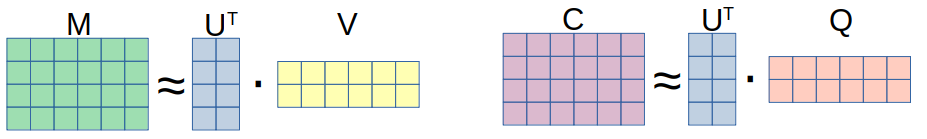
\includegraphics[width=0.8\linewidth]{images/mf2} \caption{Schematic representation of the proposed matrix co-factorization.}\label{fig:unnamed-chunk-15}
\end{figure}

Because of the non-negativity of the entries in \(M\) and \(C\), it makes sense to restrict at least \(U\) to be non-negative. This enhances the interpretability of the resulting topics (Kuang, Choo, and Park (2015), Albalawi, Yeap, and Benyoucef (2020)). So the minimization is subject to:

\begin{equation}U, V,Q \geq 0 \text{ elementwise.}\label{eq:cons}
\end{equation}

The corresponding algorithm for minimizing \eqref{eq:minc} under the constraint \eqref{eq:cons} is based on the alternating minimization/ alternating projection in from of the hierarchical non-negative alternating least squares (HALS) of Cichocki, Zdunek, and Amari (2007) with our modification for the co-factorization setup (see also Degleris et al. (2019)).

For the loss function \(J(U,V,Q)\), we have:

\begin{align*}J(U,V,Q) &= ||M-U^\top V||^2 + \lambda ||C-U^\top Q|| \\
&= ||M-\sum_{k=1}^K u_kv_k^\top||^2 + \lambda ||C-\sum_{k=1}^K u_kq_k^\top||\\
&=||M-\sum_{k\not=p} u_kv_k^\top - u_pv_p^\top||^2 + \lambda ||C-\sum_{k\not=p} u_kq_k^\top - u_pq_p^\top||\\
&= Tr((M-\sum_{k\not=p} u_kv_k^\top)^\top (M-\sum_{k\not=p} u_kv_k^\top) - 2(M-\sum_{k\not=p} u_kv_k^\top)u_pv_p^\top + u_pv_p^\top v_p u_p) + \\
&+\lambda Tr((C-\sum_{k\not=p} u_kq_k^\top)^\top (C-\sum_{k\not=p} u_kq_k^\top) - 2(C-\sum_{k\not=p} u_kq_k^\top)u_pq_p^\top + u_pq_p^\top q_p u_p).
\end{align*}

The derivative with respect to \(u_p\) is:

\[\frac{\partial J(U,V,Q)}{\partial u_p} = - 2(M-\sum_{k\not=p} u_kv_k^\top)v_p^\top + 2u_pv_p^\top v_p - 2\lambda (C-\sum_{k\not=p} u_kq_k^\top)q_p^\top + 2\lambda u_pq_p^\top q_p.\]

Hence with Karush-Kuhn-Tucker conditions for optimality:

\[u_p = \max\left(0, \frac{(M-\sum_{k\not=p} u_kv_k^\top)v_p^\top + \lambda (C-\sum_{k\not=p} u_kq_k^\top)q_p^\top)}{v_p^\top v_p + \lambda q_p^\top q_p}\right).\]

The update rules for \(v_p\) and \(q_p\) do not differ from the HALS algorithm for NMF in Cichocki, Zdunek, and Amari (2007), that is:

\[v_p = \max\left(0, \frac{u_p(M-\sum_{k\not=p} u_kv_k^\top)}{u_p^\top u_p}\right),\]

\[q_p = \max\left(0, \frac{u_p(C-\sum_{k\not=p} u_kq_k^\top)}{u_p^\top u_p}\right).\]

The resulting Algorithm 1 is presented below.

\begin{algorithm}[H]
\begin{algorithmic}
\REQUIRE $K, \lambda$
\WHILE{not converged}
\FOR{$k=1$ to $K$}
\STATE update $V_k\leftarrow \max\left(\frac{U_k(M-U_{-k}^\top V_{-k})}{U_kU_k^\top },0\right)$
\STATE update $Q_k\leftarrow \max\left(\frac{U_k(C-U_{-k}^\top Q_{-k})}{U_kU_k^\top},0\right)$
\STATE update $U_k^\top \leftarrow \max\left(\frac{(M-U_{-k}^\top V_{-k})V_k^\top + \lambda (C-U_{-k}^\top Q_{-k})Q_k^\top}{ V_k^\top V_k  + \lambda Q_k^\top Q_k },0\right)$
\ENDFOR
\ENDWHILE
\end{algorithmic}
\caption{HALS algorithm for NMCF}
\end{algorithm}

\(X_k\) denotes the \(k\)th row of the matrix \(X\) and \(X_{-k}\) denotes the matrix without its \(k\)th row.

In summary, for a given \(K\) and \(\lambda\), the algorithm delivers a common low dimensional representation of \(M\) and \(C\) optimal in the sense of minimizing \(J(U,V,Q)\) under the non-negativity condition. \(U\) represents thereby a common latent topic space and \(V,Q\) are the low dimensional embeddings for the respective contexts in the topic space. The resulting low dimensional representation of corporate reports together with SDGs create a basis for choosing, evaluating and monitoring investments with respect to their impact on society and the environment.

\hypertarget{application-of-nmcf}{%
\section{Application of NMCF}\label{application-of-nmcf}}

In this section, we apply the proposed algorithm to the bag-of-words representations of reports sections and SDG texts. The associated algorithm of NMCF requires the input of two nuisance parameter values. The first parameter \(\lambda\) governs the importance of the side information in the co-factorization procedure. The second parameter \(K\) specifies the number of latent topics and thus the resulting dimension of the latent topic space. We propose a data-driven procedure for the choice of \(K\) and \(\lambda\) based on maximizing the average topic coherence, present and visualize the resulting topic representations, and demonstrate their usefulness for sustainability assessment via two common (dis)similarity measures.

\hypertarget{choosing-lambda-and-k}{%
\subsection{\texorpdfstring{Choosing \(\lambda\) and \(K\)}{Choosing \textbackslash lambda and K}}\label{choosing-lambda-and-k}}

In order to accomplish the NMCF via the Algorithm 1, we have to specify our choice of the number of topics \(K\) (which corresponds to the dimension of the latent topic space) and the nuisance parameter \(\lambda\) of the loss function. We use a data-driven procedure to simultaneously choose \(K\) and \(\lambda\) among plausible values based on maximizing the average mean-logratio topic coherence (Thompson and Mimno (2018), Selivanov, Bickel, and Wang (2022)).

The log coherence for a topic \(k\) with \(m\) top words \(w_{k,1},\ldots, w_{k,m}\), \(coh_k\), is given as:

\begin{equation}
coh_{k}=\sum_{i=1}^m\sum_{j<i}\log\frac{\#(w_{k,i},w_{k,j})}{\#(w_{k,i})}+\varepsilon,\label{eq:coh}
\end{equation}

where \(\#(\cdot)\) counts the contexts containing the input (a word or a word pair) and \(\varepsilon\) is a smoothing parameter. This metric quantifies how often the top \(m\) words in a topic \(k\) co-occur in the reference text corpus. It is justified by the observation that words with similar meaning tend to co-occur in the same contexts. That is, coherence of a topic is positively associated with its interpretability.

\begin{figure}
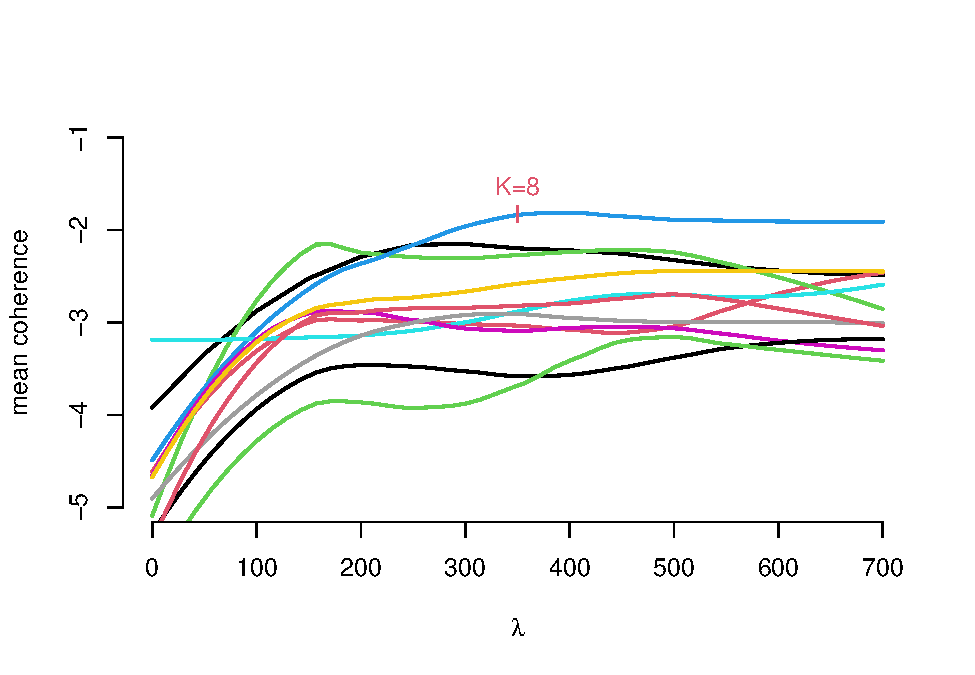
\includegraphics[width=0.8\linewidth]{20240314_sustain_dim_files/figure-latex/figtraj-1} \caption{The trajectories for the average coherence for different choices of \(K=5,6,\ldots,15\) and \(\lambda\in [0,700]\).}\label{fig:figtraj}
\end{figure}

To find the optimal values for the nuisance parameters in the sense of maximum topic coherence, we create the meaningful combinations of \(K\) and \(\lambda\) with \(K=5,\ldots,15\) and \(\lambda\in[0,700],\) apply the NMCF algorithm to our data, and compute the log coherence for each topic as defined in \eqref{eq:coh}. We subsequently average the coherence measures over all topics:

\begin{equation}
\overline{coh}=\frac 1k \sum_{k=1}^Kcoh_k.\label{eq:acoh}
\end{equation}

The resulting trajectories for different \(K\) and \(\lambda\) are shown in Figure \ref{fig:figtraj}. Finally, we choose the combination of \(K\) and \(\lambda\) which results in the highest average log coherence computed by \eqref{eq:acoh}. The optimal nuisance parameters for our data is therefore the number of topics \(K=8\) combined with the importance parameter \(\lambda=350.\)

\hypertarget{results}{%
\subsection{Results}\label{results}}

The output of Algorithm 1 are the decomposition matrices \(V,U\) and \(Q\). \(U\) contains the term-topic representations. By looking at the largest entries of \(U\) and the corresponding terms (the top words), we can interpret the resulting latent topics. The entries of \(V,Q\) and their relative magnitudes reveal the proportions (or the importance) of the topics in the text corpus.

\begin{figure}
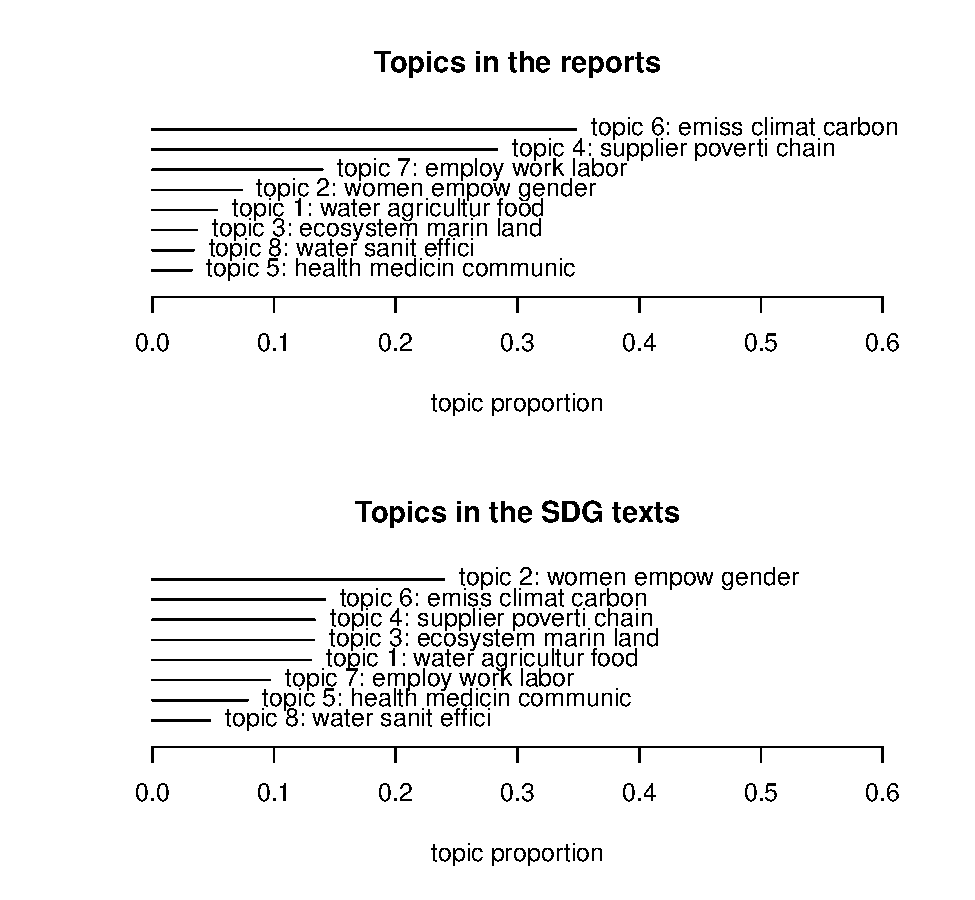
\includegraphics[width=0.8\linewidth]{20240314_sustain_dim_files/figure-latex/figtpropg-1} \caption{Topic proportion and the words with the highest weight per topic for each of the discovered topics in the reports (top) and in the SDG texts (bottom).}\label{fig:figtpropg}
\end{figure}

Figure \ref{fig:figtpropg} shows the topic proportions and the words with the highest weight per topic for each of the discovered topics in the reports texts and the SGD texts respectively. The top three words shown already allow to interpret the topics. The distribution of the topics is somewhat different in the report texts compared to the SDG texts. The topics ``emiss climate carbon'' and ``supplier poverti chain'' become a large share in the distribution in both reports and SDGs. Whereas the topic ``women empow gender'' seem to dominate the SDGs, it gains relatively low importance in the reports. By using this kind of representation new action areas for the companies can be discovered.

The entries of \(V\) and \(Q\) deliver the \(k\)-dimensional context-topic representations enabling us to compare the underlying contexts in a low dimensional topic space using the embeddings of the contexts, which correspond to the entries of \(V\) and \(Q\).
Using the obtained representations of corporate reports together with the SDGs in the following, we show a couple of strategies for choosing, evaluating and monitoring investments with respect to their impact on society and the environment in the next subsection.

\hypertarget{associating-the-reports-with-the-sdgs}{%
\subsection{Associating the reports with the SDGs}\label{associating-the-reports-with-the-sdgs}}

Now we employ two different (dis)similarity measures to associate the reports to the SDGs. We associate the reports using one common dissimilarity measure - the Euclidean distance, and one common similarity measure - the cosine similarity. Since in our analysis each report is a combination of several contexts, each represented in a \(8\)-dimensional topic space, we need to aggregate the (dis)similarity measures used to a report level. As a result, for the Euclidean distance we choose the minimum, and for the cosine similarity - the maximum for the aggregation over all contexts to the report level.

In the upper panel of Figure \ref{fig:figcos}, we use the normalized minimum Euclidean distance to compare the reports with the SDGs. Therefore we first compute the Euclidean distance between each context (report section) and the SDG texts and then take the minimum of the distance over all contexts of each report as the resulting dissimilarity measure to a particular goal. In the lower panel of Figure \ref{fig:figcos}, we use the maximum cosine similarity for each report in order to associate its contents to the SDGs. Similary to the minimum Euclidean distance, we first compute the cosine similarity between each context of a report and each SDG, and then take the maximum over all report contexts as the resulting similarity measure.

\begin{figure}
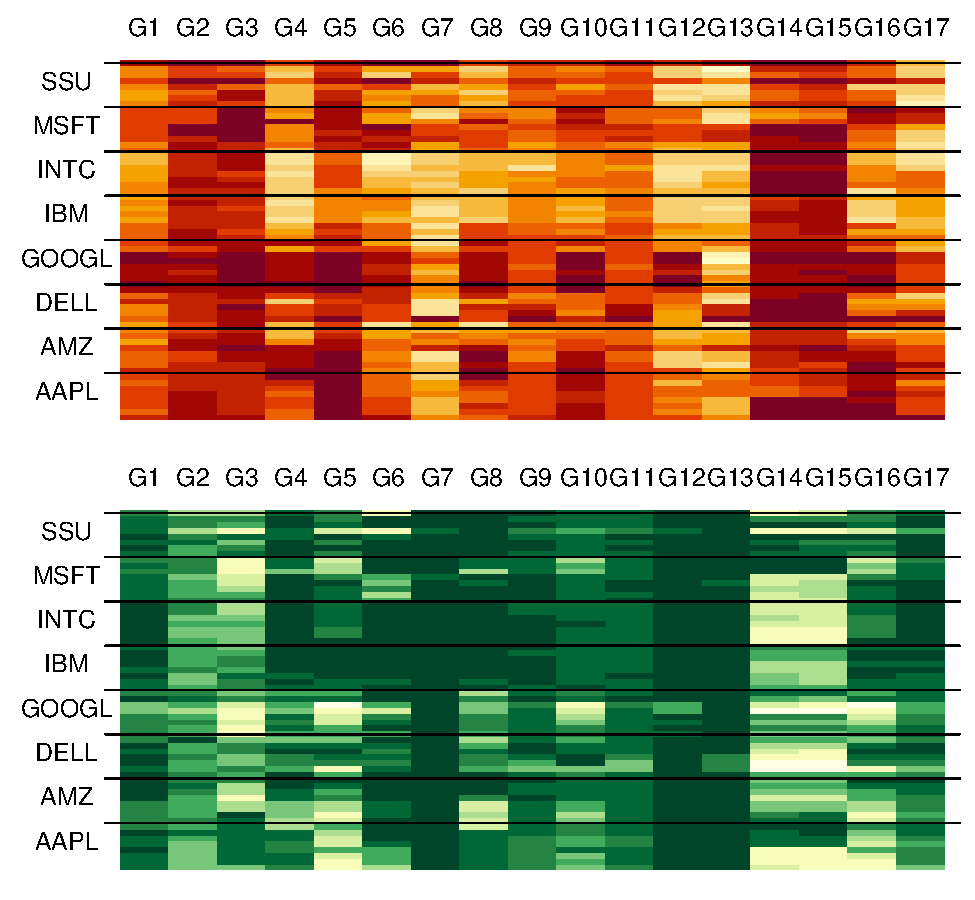
\includegraphics[width=0.8\linewidth]{20240314_sustain_dim_files/figure-latex/figcos-1} \caption{(Dis)similarity measures between the reports over the available company-years (rows, starting with earlier years on the top) and the SDGs (columns) computed using the resulting topic embeddings.  Upper panel: normalized minimum Euclidean distance (Lighter colors correspond to smaller distances.). Lower panel: maximum cosine similarity (Darker colors correspond to higher similarity values.).}\label{fig:figcos}
\end{figure}

Note, that the (dis)similarity measures in Figure \ref{fig:figcos} are computed for each company-year enabling dynamic analysis of the underlying SDG related content and the associated progress in company sustainability actions evolution over time.

For a static analysis, we can use the \emph{average} the dissimilarities over the all available report years and construct a dissimilarity-based rating of the considered firms with respect to each of the SDGs. The associated dissimilarity-based rating is presented in Table \ref{tab:tab01}.

\begin{table}

\caption{\label{tab:tab01}Company dissimilarity-based rating (from the closest to the farthest) with respect to the individual SDGs unsing the obtained topic embeddings.}
\centering
\begin{tabular}[t]{l|l}
\hline
Goal & Rating\\
\hline
Goal\_1 & INTC, AMZ, SSU, DELL, IBM, AAPL, MSFT, GOOGL\\
\hline
Goal\_2 & SSU, AMZ, DELL, INTC, AAPL, MSFT, IBM, GOOGL\\
\hline
Goal\_3 & SSU, INTC, IBM, AAPL, AMZ, DELL, MSFT, GOOGL\\
\hline
Goal\_4 & INTC, SSU, AMZ, IBM, MSFT, DELL, AAPL, GOOGL\\
\hline
Goal\_5 & INTC, AMZ, IBM, SSU, DELL, MSFT, AAPL, GOOGL\\
\hline
Goal\_6 & INTC, AMZ, SSU, IBM, AAPL, DELL, MSFT, GOOGL\\
\hline
Goal\_7 & IBM, INTC, AAPL, DELL, MSFT, GOOGL, AMZ, SSU\\
\hline
Goal\_8 & INTC, SSU, AMZ, MSFT, DELL, IBM, AAPL, GOOGL\\
\hline
Goal\_9 & INTC, AMZ, MSFT, IBM, SSU, GOOGL, AAPL, DELL\\
\hline
Goal\_10 & INTC, AMZ, SSU, DELL, IBM, MSFT, AAPL, GOOGL\\
\hline
Goal\_11 & INTC, MSFT, AMZ, AAPL, IBM, GOOGL, SSU, DELL\\
\hline
Goal\_12 & INTC, SSU, AMZ, IBM, AAPL, DELL, MSFT, GOOGL\\
\hline
Goal\_13 & INTC, GOOGL, SSU, AMZ, AAPL, IBM, MSFT, DELL\\
\hline
Goal\_14 & SSU, MSFT, AAPL, AMZ, IBM, INTC, GOOGL, DELL\\
\hline
Goal\_15 & SSU, MSFT, AMZ, AAPL, IBM, INTC, GOOGL, DELL\\
\hline
Goal\_16 & INTC, AMZ, DELL, IBM, SSU, MSFT, AAPL, GOOGL\\
\hline
Goal\_17 & SSU, INTC, IBM, MSFT, AMZ, DELL, GOOGL, AAPL\\
\hline
\end{tabular}
\end{table}

Similar, by averaging the cosine similarities for a company over all available report years, we construct a similarity-based rating of the considered firms with respect to each of the SDGs. The rating is presented in Table \ref{tab:tab02}.

\begin{table}

\caption{\label{tab:tab02}Company similarity-based rating (from the most similar to the least similar) with respect to the individual SDGs using the obtained topic embeddings.}
\centering
\begin{tabular}[t]{l|l}
\hline
Goal & Rating\\
\hline
Goal\_1 & INTC, AMZ, DELL, SSU, IBM, AAPL, MSFT, GOOGL\\
\hline
Goal\_2 & AMZ, MSFT, GOOGL, IBM, SSU, DELL, INTC, AAPL\\
\hline
Goal\_3 & AAPL, IBM, DELL, SSU, INTC, AMZ, MSFT, GOOGL\\
\hline
Goal\_4 & INTC, AMZ, SSU, MSFT, IBM, DELL, GOOGL, AAPL\\
\hline
Goal\_5 & INTC, IBM, AMZ, SSU, DELL, MSFT, GOOGL, AAPL\\
\hline
Goal\_6 & INTC, AMZ, IBM, AAPL, DELL, SSU, MSFT, GOOGL\\
\hline
Goal\_7 & AMZ, IBM, AAPL, GOOGL, INTC, DELL, MSFT, SSU\\
\hline
Goal\_8 & SSU, INTC, AMZ, MSFT, IBM, DELL, AAPL, GOOGL\\
\hline
Goal\_9 & INTC, IBM, AMZ, MSFT, SSU, GOOGL, AAPL, DELL\\
\hline
Goal\_10 & INTC, IBM, AMZ, SSU, DELL, MSFT, AAPL, GOOGL\\
\hline
Goal\_11 & IBM, INTC, MSFT, SSU, AMZ, GOOGL, AAPL, DELL\\
\hline
Goal\_12 & IBM, INTC, AMZ, AAPL, SSU, DELL, MSFT, GOOGL\\
\hline
Goal\_13 & AMZ, IBM, INTC, GOOGL, AAPL, SSU, MSFT, DELL\\
\hline
Goal\_14 & SSU, IBM, AAPL, MSFT, AMZ, GOOGL, INTC, DELL\\
\hline
Goal\_15 & SSU, AAPL, IBM, MSFT, AMZ, GOOGL, INTC, DELL\\
\hline
Goal\_16 & INTC, IBM, SSU, AMZ, DELL, MSFT, GOOGL, AAPL\\
\hline
Goal\_17 & INTC, SSU, IBM, MSFT, AMZ, DELL, GOOGL, AAPL\\
\hline
\end{tabular}
\end{table}

\begin{verbatim}
## [1] 0.2030812
\end{verbatim}

Though positively correlated (mean rank correlation is \(0.2031\)), the two ratings exhibit noticeable differences. Therefore, a suitable (dis)similarity measure should be chosen carefuly. Since cosine similarity is shown to perform better than Euclidean distance in text comparison tasks (see i.e. Alobed, Altrad, and Bakar (2021)), the usage of cosine similarity in our association analysis is more inline with the main-stream text mining literature.

In our framework, we are not restricted to associating the reports to the individual SDGs only. We are also able to consider any linear combinations of the goals composed based on personal preferences, such that, in a sense, a personalized sustainability goal for a tailored sustainability assessment can be easily created. In order to considering individual preferences, let us define a linear combination of the goals using weights \(\beta=(\beta_1,\ldots,\beta_{17})^\top\). Then \(C\beta\approx UQ^\top\beta\) defines a ``personalized'' goal based on the term occurrences approximated by the co-factorization. Using the following four different combinations (portfolios) of SDGs, we provide an example of such tailored sustainability assessment.

Our example portfolios are:

\begin{itemize}
\tightlist
\item
  ``all\_equal'' (all goals are equally weighted),
\item
  ``basic\_needs'' (the goals addressing the basic human needs (SDGs 1-6) are equally weighted and all other goals have zero weights),
\item
  ``fair\_society'' (the goals concerning society and infrastructure developement (SDGs 7-12 and 16-17) are equaly weighted and all other goals have zero weights),
\item
  ``climate\_life'' (the goals addressing climate, plant and animal life (SDGs 13-15) are equally weighted and all other goals have zero weights).
\end{itemize}

\begin{table}

\caption{\label{tab:tab03}Company rating (from closest to farthest) with respect to the individual SDG combination based on the average Euclidean distance of the report embeddings in year 2022.}
\centering
\begin{tabular}[t]{l|l}
\hline
goal & rating\\
\hline
all\_equal & INTC, DELL, AMZ, IBM, MSFT, SSU, AAPL, GOOGL\\
\hline
basic\_needs & AMZ, INTC, DELL, IBM, AAPL, SSU, MSFT, GOOGL\\
\hline
fair\_society & DELL, INTC, AMZ, MSFT, IBM, AAPL, SSU, GOOGL\\
\hline
climate\_life & MSFT, IBM, AMZ, INTC, AAPL, DELL, GOOGL, SSU\\
\hline
\end{tabular}
\end{table}

In Table \ref{tab:tab03}, the resulting firm rating based on each SDG portfolio is presented. As shown, the ratings can be quite different depending on the concrete preferences. In general, any linear combination of the goals can build a basis for such a comparison. This makes the proposed procedure very flexible. Moreover, any user defined (dis)similarity metric can be applied to the resulting embeddings in the topic space, which grant additional flexibility to our method.

In summary, as shown in the above analysis, the proposed matrix co-factorization for sustainability assessment with respect to the predefined structure of the 17 SDGs, is a transparent and flexible approach resulting in a low dimensional topic representation facilitating adaptive association of the sustainability related reports with the SDGs.

\hypertarget{conclusion-and-discussion}{%
\section{Conclusion and Discussion}\label{conclusion-and-discussion}}

As shown in Aureli et al. (2020), sustainability related disclosures have significant impact on company value. That is, the contained information influences investor reactions and subsequent pricing. This shows an increasing importance of incorporating this textual information into sustainability analysis. To insure both objectivity and flexibility of the analysis, we propose a simple approach enabling us to represent the textual content of the reports in a topic space using the 17 SDGs as a predefined structure.

The proposed methodology builds upon a non-negative matrix co-factorization for topic extraction with side information, which results in a low dimensional representation in a prestructured topic space. The method is scalable, simple to implement, computationally efficient and does not require any manual intervention as other comparable methods. It delivers transparent and interpretable results with many use cases.

The adopted matrix co-factorization jointly factorizes two term-context matrices: the first one containing the term-contexts counts for the corpus of sustainability related reports and the second one containing the term-context counts for the SDG texts, which represents the predefined structure or the side information in our context. The associated algorithm based on hierarchical NMF requires the input of two nuisance parameter values. The first nuisance parameter \(\lambda\) governs the importance of the side information in the co-factorization procedure. The second nuisance parameter \(K\) specifies the number of latent topics and thus the resulting dimension of the latent topic space. We provide a data driven procedure for choosing the values of the nuisance parameters by maximizing the common goodness-of-fit measure for an unsupervised topic extraction: the average topic coherence.

The resulting contextual embeddings in a low dimensional topic space build a basis for dynamic comparison of the sustainability related reports for eight listed tech firms. We associate the reports using one dissimilarity measure - minimum Euclidean distance, and one similarity measure - maximum cosine similarity. The results show, that our procedure can efficiently assists financial decisions under tailored SDGs based preferences.

Nevertheless, an important premise of our analysis, that the reports texts contain objective information on firms' sustainability actions, may not hold in general. Laskin and Nesova (2022) discuss the issue of credibility of sustainability reports and point out a bias towards the optimistic language. Moreover, we do not take into consideration the sentiment associated with the report content (positive or negative tone), which is an important aspect of sustainability assessment (Mućko (2021)). Incorporation of these issues in the analysis is a promising subject for future research.

\hypertarget{references}{%
\section*{References}\label{references}}
\addcontentsline{toc}{section}{References}

\hypertarget{refs}{}
\begin{CSLReferences}{1}{0}
\leavevmode\vadjust pre{\hypertarget{ref-albalawi2020}{}}%
Albalawi, Rania, Tet Hin Yeap, and Morad Benyoucef. 2020. {``Using Topic Modeling Methods for Short-Text Data: A Comparative Analysis.''} \emph{Frontiers in Artificial Intelligence} 3. \url{https://doi.org/10.3389/frai.2020.00042}.

\leavevmode\vadjust pre{\hypertarget{ref-alobed2021}{}}%
Alobed, Mohammad, Abdallah M M Altrad, and Zainab Binti Abu Bakar. 2021. {``A Comparative Analysis of Euclidean, Jaccard and Cosine Similarity Measure and Arabic Wordnet for Automated Arabic Essay Scoring.''} In \emph{2021 Fifth International Conference on Information Retrieval and Knowledge Management (CAMP)}, 70--74. \url{https://doi.org/10.1109/CAMP51653.2021.9498119}.

\leavevmode\vadjust pre{\hypertarget{ref-amini2018}{}}%
Amini, Mehdi, Carol C. Bienstock, and John A. Narcum. 2018. {``Status of Corporate Sustainability: A Content Analysis of Fortune 500 Companies.''} \emph{Business Strategy and the Environment} 27 (8): 1450--61. https://doi.org/\url{https://doi.org/10.1002/bse.2195}.

\leavevmode\vadjust pre{\hypertarget{ref-aureli2020}{}}%
Aureli, Selena, Sabrina Gigli, Renato Medei, and Enrico Supino. 2020. {``The Value Relevance of Environmental, Social, and Governance Disclosure: Evidence from Dow Jones Sustainability World Index Listed Companies.''} \emph{Corporate Social Responsibility and Environmental Management} 27 (1): 43--52. https://doi.org/\url{https://doi.org/10.1002/csr.1772}.

\leavevmode\vadjust pre{\hypertarget{ref-quanteda}{}}%
Benoit, Kenneth, Kohei Watanabe, Haiyan Wang, Paul Nulty, Adam Obeng, Stefan Müller, and Akitaka Matsuo. 2018. {``Quanteda: An r Package for the Quantitative Analysis of Textual Data.''} \emph{Journal of Open Source Software} 3 (30): 774. \url{https://doi.org/10.21105/joss.00774}.

\leavevmode\vadjust pre{\hypertarget{ref-berg2022}{}}%
Berg, Florian, Julian F Kölbel, and Roberto Rigobon. 2022. {``{Aggregate Confusion: The Divergence of ESG Ratings*}.''} \emph{Review of Finance} 26 (6): 1315--44. \url{https://doi.org/10.1093/rof/rfac033}.

\leavevmode\vadjust pre{\hypertarget{ref-blei2003}{}}%
Blei, David M., Andrew Y. Ng, and Michael I. Jordan. 2003. {``Latent Dirichlet Allocation.''} \emph{J. Mach. Learn. Res.} 3 (null): 993--1022.

\leavevmode\vadjust pre{\hypertarget{ref-chen2023}{}}%
Chen, Weisi, Fethi Rabhi, Wenqi Liao, and Islam Al-Qudah. 2023. {``Leveraging State-of-the-Art Topic Modeling for News Impact Analysis on Financial Markets: A Comparative Study.''} \emph{Electronics} 12 (12). \url{https://doi.org/10.3390/electronics12122605}.

\leavevmode\vadjust pre{\hypertarget{ref-CHEN2019}{}}%
Chen, Yong, Hui Zhang, Rui Liu, Zhiwen Ye, and Jianying Lin. 2019. {``Experimental Explorations on Short Text Topic Mining Between LDA and NMF Based Schemes.''} \emph{Knowledge-Based Systems} 163: 1--13. https://doi.org/\url{https://doi.org/10.1016/j.knosys.2018.08.011}.

\leavevmode\vadjust pre{\hypertarget{ref-chen2017}{}}%
Chen, Yu, Rhaad M. Rabbani, Aparna Gupta, and Mohammed J. Zaki. 2017. {``Comparative Text Analytics via Topic Modeling in Banking.''} In \emph{2017 IEEE Symposium Series on Computational Intelligence (SSCI)}, 1--8. \url{https://doi.org/10.1109/SSCI.2017.8280945}.

\leavevmode\vadjust pre{\hypertarget{ref-churchill2022}{}}%
Churchill, Rob, and Lisa Singh. 2022. {``The Evolution of Topic Modeling.''} \emph{ACM Comput. Surv.} 54 (10s). \url{https://doi.org/10.1145/3507900}.

\leavevmode\vadjust pre{\hypertarget{ref-cichocki2007}{}}%
Cichocki, Andrzej, Rafal Zdunek, and Shun-ichi Amari. 2007. {``Hierarchical ALS Algorithms for Nonnegative Matrix and 3D Tensor Factorization.''} In \emph{Independent Component Analysis and Signal Separation}, edited by Mike E. Davies, Christopher J. James, Samer A. Abdallah, and Mark D. Plumbley, 169--76. Berlin, Heidelberg: Springer Berlin Heidelberg.

\leavevmode\vadjust pre{\hypertarget{ref-deerwester1990}{}}%
Deerwester, Scott, Susan T. Dumais, George W. Furnas, Thomas K. Landauer, and Richard Harshman. 1990. {``Indexing by Latent Semantic Analysis.''} \emph{Journal of the American Society for Information Science} 41 (6): 391--407. https://doi.org/\url{https://doi.org/10.1002/(SICI)1097-4571(199009)41:6\%3C391::AID-ASI1\%3E3.0.CO;2-9}.

\leavevmode\vadjust pre{\hypertarget{ref-degleris2019}{}}%
Degleris, Anthony, Ben Antin, Surya Ganguli, and Alex H Williams. 2019. {``Fast Convolutive Nonnegative Matrix Factorization Through Coordinate and Block Coordinate Updates.''} \url{https://arxiv.org/abs/1907.00139}.

\leavevmode\vadjust pre{\hypertarget{ref-egger2022}{}}%
Egger, Roman, and Joanne Yu. 2022. {``A Topic Modeling Comparison Between LDA, NMF, Top2Vec, and BERTopic to Demystify Twitter Posts.''} \emph{Frontiers in Sociology} 7. \url{https://doi.org/10.3389/fsoc.2022.886498}.

\leavevmode\vadjust pre{\hypertarget{ref-eshima2023}{}}%
Eshima, Shusei, Kosuke Imai, and Tomoya Sasaki. 2023. {``Keyword Assisted Topic Models.''} \url{https://arxiv.org/abs/2004.05964}.

\leavevmode\vadjust pre{\hypertarget{ref-fang2011}{}}%
Fang, Yi, and Luo Si. 2011. {``Matrix Co-Factorization for Recommendation with Rich Side Information and Implicit Feedback.''} In \emph{Proceedings of the 2nd International Workshop on Information Heterogeneity and Fusion in Recommender Systems}, 65--69. HetRec '11. New York, NY, USA: Association for Computing Machinery. \url{https://doi.org/10.1145/2039320.2039330}.

\leavevmode\vadjust pre{\hypertarget{ref-figuera2024}{}}%
Figuera, Pau, and Pablo García Bringas. 2024. {``Revisiting Probabilistic Latent Semantic Analysis: Extensions, Challenges and Insights.''} \emph{Technologies} 12 (1). \url{https://doi.org/10.3390/technologies12010005}.

\leavevmode\vadjust pre{\hypertarget{ref-gupta2020}{}}%
Gupta, Aaryan, Vinya Dengre, Hamza Abubakar Kheruwala, and Manan Shah. 2020. {``Comprehensive Review of Text-Mining Applications in Finance.''} \emph{Financial Innovation} 6 (1): 1--25. \url{https://doi.org/10.1186/s40854-020-00205-1}.

\leavevmode\vadjust pre{\hypertarget{ref-Harandizadeh2022}{}}%
Harandizadeh, Bahareh, J. Hunter Priniski, and Fred Morstatter. 2022. {``Keyword Assisted Embedded Topic Model.''} In \emph{Proceedings of the Fifteenth {ACM} International Conference on Web Search and Data Mining}. {ACM}. \url{https://doi.org/10.1145/3488560.3498518}.

\leavevmode\vadjust pre{\hypertarget{ref-hofmann1999}{}}%
Hofmann, Thomas. 1999. {``Probabilistic Latent Semantic Indexing.''} In \emph{Proceedings of the 22nd Annual International ACM SIGIR Conference on Research and Development in Information Retrieval}, 50--57. SIGIR '99. New York, NY, USA: Association for Computing Machinery. \url{https://doi.org/10.1145/312624.312649}.

\leavevmode\vadjust pre{\hypertarget{ref-kang2022}{}}%
Kang, Hyewon, and Jinho Kim. 2022. {``Analyzing and Visualizing Text Information in Corporate Sustainability Reports Using Natural Language Processing Methods.''} \emph{Applied Sciences} 12 (11). \url{https://doi.org/10.3390/app12115614}.

\leavevmode\vadjust pre{\hypertarget{ref-Kuang2015}{}}%
Kuang, Da, Jaegul Choo, and Haesun Park. 2015. {``Nonnegative Matrix Factorization for Interactive Topic Modeling and Document Clustering.''} In \emph{Partitional Clustering Algorithms}, edited by M. Emre Celebi, 215--43. Cham: Springer International Publishing. \url{https://doi.org/10.1007/978-3-319-09259-1_7}.

\leavevmode\vadjust pre{\hypertarget{ref-landrum2018}{}}%
Landrum, Nancy, and Brian Ohsowski. 2017. {``Identifying Worldviews on Corporate Sustainability: A Content Analysis of Corporate Sustainability Reports.''} \emph{Business Strategy and the Environment} 27 (November). \url{https://doi.org/10.1002/bse.1989}.

\leavevmode\vadjust pre{\hypertarget{ref-laskin2022}{}}%
Laskin, Alexander V., and Natalya Mikhailovna Nesova. 2022. {``The Language of Optimism in Corporate Sustainability Reports: A Computerized Content Analysis.''} \emph{Business and Professional Communication Quarterly} 85 (1): 80--98. \url{https://doi.org/10.1177/23294906211065507}.

\leavevmode\vadjust pre{\hypertarget{ref-lee2000}{}}%
Lee, Daniel, and H. Sebastian Seung. 2000. {``Algorithms for Non-Negative Matrix Factorization.''} In \emph{Advances in Neural Information Processing Systems}, edited by T. Leen, T. Dietterich, and V. Tresp. Vol. 13. MIT Press. \url{https://proceedings.neurips.cc/paper_files/paper/2000/file/f9d1152547c0bde01830b7e8bd60024c-Paper.pdf}.

\leavevmode\vadjust pre{\hypertarget{ref-LI2017}{}}%
Li, Guowen, Xiaoqian Zhu, Jun Wang, Dengsheng Wu, and Jianping Li. 2017. {``Using LDA Model to Quantify and Visualize Textual Financial Stability Report.''} \emph{Procedia Computer Science} 122: 370--76. https://doi.org/\url{https://doi.org/10.1016/j.procs.2017.11.382}.

\leavevmode\vadjust pre{\hypertarget{ref-LIEW2014}{}}%
Liew, Wan Te, Arief Adhitya, and Rajagopalan Srinivasan. 2014. {``Sustainability Trends in the Process Industries: A Text Mining-Based Analysis.''} \emph{Computers in Industry} 65 (3): 393--400. https://doi.org/\url{https://doi.org/10.1016/j.compind.2014.01.004}.

\leavevmode\vadjust pre{\hypertarget{ref-loughran2016}{}}%
Loughran, Tim, and Bill McDonald. 2016. {``Textual Analysis in Accounting and Finance: A Survey.''} \emph{Journal of Accounting Research} 54 (4): 1187--1230. https://doi.org/\url{https://doi.org/10.1111/1475-679X.12123}.

\leavevmode\vadjust pre{\hypertarget{ref-luo2019}{}}%
Luo, Ling, Haoran Xie, Yanghui Rao, and Fu Lee Wang. 2019. {``Personalized Recommendation by Matrix Co-Factorization with Tags and Time Information.''} \emph{Expert Systems with Applications} 119: 311--21. https://doi.org/\url{https://doi.org/10.1016/j.eswa.2018.11.003}.

\leavevmode\vadjust pre{\hypertarget{ref-MUCKO2021}{}}%
Mućko, Przemysław. 2021. {``Sentiment Analysis of CSR Disclosures in Annual Reports of EU Companies.''} \emph{Procedia Computer Science} 192: 3351--59. https://doi.org/\url{https://doi.org/10.1016/j.procs.2021.09.108}.

\leavevmode\vadjust pre{\hypertarget{ref-NUGUMANOVA2022}{}}%
Nugumanova, Aliya, Darkhan Akhmed-Zaki, Madina Mansurova, Yerzhan Baiburin, and Almasbek Maulit. 2022. {``NMF-Based Approach to Automatic Term Extraction.''} \emph{Expert Systems with Applications} 199: 117179. https://doi.org/\url{https://doi.org/10.1016/j.eswa.2022.117179}.

\leavevmode\vadjust pre{\hypertarget{ref-rr}{}}%
R Core Team. 2023. \emph{R: A Language and Environment for Statistical Computing}. Vienna, Austria: R Foundation for Statistical Computing. \url{https://www.R-project.org/}.

\leavevmode\vadjust pre{\hypertarget{ref-rao2015}{}}%
Rao, Nikhil, Hsiang-Fu Yu, Pradeep K Ravikumar, and Inderjit S Dhillon. 2015. {``Collaborative Filtering with Graph Information: Consistency and Scalable Methods.''} In \emph{Advances in Neural Information Processing Systems}, edited by C. Cortes, N. Lawrence, D. Lee, M. Sugiyama, and R. Garnett. Vol. 28. Curran Associates, Inc. \url{https://proceedings.neurips.cc/paper_files/paper/2015/file/f4573fc71c731d5c362f0d7860945b88-Paper.pdf}.

\leavevmode\vadjust pre{\hypertarget{ref-text2vec}{}}%
Selivanov, Dmitriy, Manuel Bickel, and Qing Wang. 2022. \emph{Text2vec: Modern Text Mining Framework for r}. \url{https://CRAN.R-project.org/package=text2vec}.

\leavevmode\vadjust pre{\hypertarget{ref-soh2014}{}}%
Soh, Dominic S. B. 2014. {``Sustainability Reporting and Assurance: A Historical Analysis on a World-Wide Phenomenon.''} \emph{Social and Environmental Accountability Journal} 34 (2): 125--25. \url{https://doi.org/10.1080/0969160X.2014.938484}.

\leavevmode\vadjust pre{\hypertarget{ref-SULEMAN2021}{}}%
Suleman, Raja Muhammad, and Ioannis Korkontzelos. 2021. {``Extending Latent Semantic Analysis to Manage Its Syntactic Blindness.''} \emph{Expert Systems with Applications} 165: 114130. https://doi.org/\url{https://doi.org/10.1016/j.eswa.2020.114130}.

\leavevmode\vadjust pre{\hypertarget{ref-thompson-mimno-2018}{}}%
Thompson, Laure, and David Mimno. 2018. {``Authorless Topic Models: Biasing Models Away from Known Structure.''} In \emph{Proceedings of the 27th International Conference on Computational Linguistics}, edited by Emily M. Bender, Leon Derczynski, and Pierre Isabelle, 3903--14. Santa Fe, New Mexico, USA: Association for Computational Linguistics. \url{https://aclanthology.org/C18-1329}.

\leavevmode\vadjust pre{\hypertarget{ref-tsalis2020}{}}%
Tsalis, Thomas A., Kyveli E. Malamateniou, Dimitrios Koulouriotis, and Ioannis E. Nikolaou. 2020. {``New Challenges for Corporate Sustainability Reporting: United Nations' 2030 Agenda for Sustainable Development and the Sustainable Development Goals.''} \emph{Corporate Social Responsibility and Environmental Management} 27 (4): 1617--29. https://doi.org/\url{https://doi.org/10.1002/csr.1910}.

\leavevmode\vadjust pre{\hypertarget{ref-vangara2020}{}}%
Vangara, Raviteja, Erik Skau, Gopinath Chennupati, Hristo Djidjev, Thomas Tierney, James P. Smith, Manish Bhattarai, Valentin G. Stanev, and Boian S. Alexandrov. 2020. {``Semantic Nonnegative Matrix Factorization with Automatic Model Determination for Topic Modeling.''} In \emph{2020 19th IEEE International Conference on Machine Learning and Applications (ICMLA)}, 328--35. \url{https://doi.org/10.1109/ICMLA51294.2020.00060}.

\leavevmode\vadjust pre{\hypertarget{ref-watanabe2022}{}}%
Watanabe, Kohei, and Yuan Zhou. 2022. {``Theory-Driven Analysis of Large Corpora: Semisupervised Topic Classification of the UN Speeches.''} \emph{Social Science Computer Review} 40 (2): 346--66. \url{https://doi.org/10.1177/0894439320907027}.

\leavevmode\vadjust pre{\hypertarget{ref-Yang2015}{}}%
Yang, Qingquan, and Weijiang Li. 2015/07. {``The LDA Topic Model Extension Study.''} In \emph{Proceedings of the International Conference on Logistics, Engineering, Management and Computer Science}, 857--60. Atlantis Press. \url{https://doi.org/10.2991/lemcs-15.2015.169}.

\leavevmode\vadjust pre{\hypertarget{ref-zahng2020_graph}{}}%
Zhang, Yupei, Yue Yun, Huan Dai, Jiaqi Cui, and Xuequn Shang. 2020. {``Graphs Regularized Robust Matrix Factorization and Its Application on Student Grade Prediction.''} \emph{Applied Sciences} 10 (5). \url{https://doi.org/10.3390/app10051755}.

\leavevmode\vadjust pre{\hypertarget{ref-Zhao2021}{}}%
Zhao, He, Dinh Q. Phung, Viet Huynh, Yuan Jin, Lan Du, and Wray L. Buntine. 2021. {``Topic Modelling Meets Deep Neural Networks: A Survey.''} In \emph{International Joint Conference on Artificial Intelligence}. \url{https://api.semanticscholar.org/CorpusID:232076325}.

\end{CSLReferences}

\end{document}
